% Template per la presentazione di laurea
%
% Creato da Giulio Spinozzi
% giuliospinozzi@gmail.com
% http://giuliospinozzi.altervista.org
%
%\makeatletter\let\ifGm@compatii\relax\makeatother %per un bug corrente, da togliere successivamente
\documentclass[12pt, hyperref={bookmarksnumbered=true}]{beamer} %Classe documento, font, segnalibri
\let\Tiny=\tiny	%Ridimensionamento del font, per un corretto rendering
\usepackage{greenAmsterdam}	%Carica il tema
\usepackage{color}	%Per usare colori aggiuntivi
\setbeamercovered{transparent}	%Effetto trasparente delle scritte
%\pgfdeclareimage[height=1.5cm]{logo}{img/logo.png}
\usepackage[latin1]{inputenc}
\usepackage{multimedia}


\title{Generazione automatica di word cloud dinamiche}
%\titlegraphic{\pgfuseimage{logo}}
\subtitle{Ingegneria Informatica e dell'Automazione \vspace{0.5cm}
\\\textsc{\textcolor[rgb]{0.00,0.00,0.00} {Universit� degli Studi di Perugia \\Facolt� di Ingegneria}}}
\author{\textbf{Candidato}: \textit{Enrico Spataro} \hspace{0.3cm} \\
\hspace{0.77cm}\textbf{Relatore}: \textit{Prof.ssa Carla Binucci}  \\
\hspace{0.55cm}\textbf{Relatore}: \textit{Prof. Walter Didimo}}
\date{\scriptsize 19.02.2016}

\begin{document}

\frame{\titlepage}	%Ogni slide � racchiusa dal tag frame

\section[Sommario]{}
\frame{
\frametitle{\textbf{Contenuti}}
\tableofcontents
}


\section{Introduzione}
\frame{
\frametitle{\textbf{Obiettivi}}
\begin{beamerboxesrounded}{}
Mostrare l'evoluzione di un testo tramite:
\begin{itemize}
\item creazione word cloud semantiche ad intervalli regolari;
\item animazioni tramite morphing.
\end{itemize}
\end{beamerboxesrounded}
}

\frame{
\frametitle{\textbf{Cos'� una word cloud?}}
\begin{center}
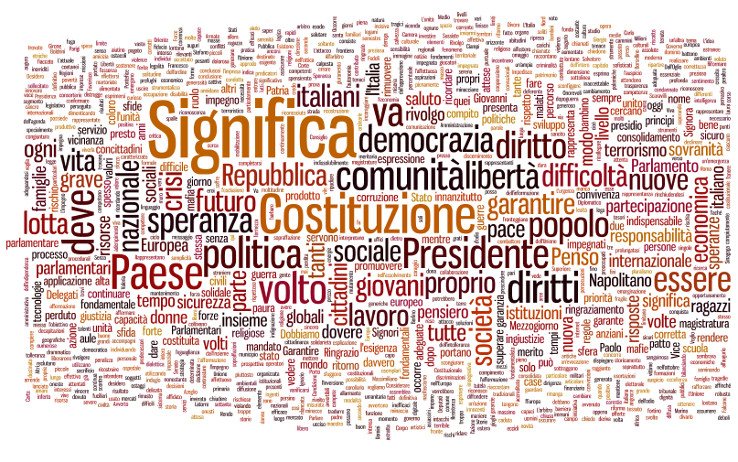
\includegraphics[scale=0.4]{img/wc_statiche/mattarella_wc.png}
\end{center}
}

\frame{
\frametitle{\textbf{Word cloud semantiche}\hspace{1mm}{\small(Kobourov et al., 2014)}}
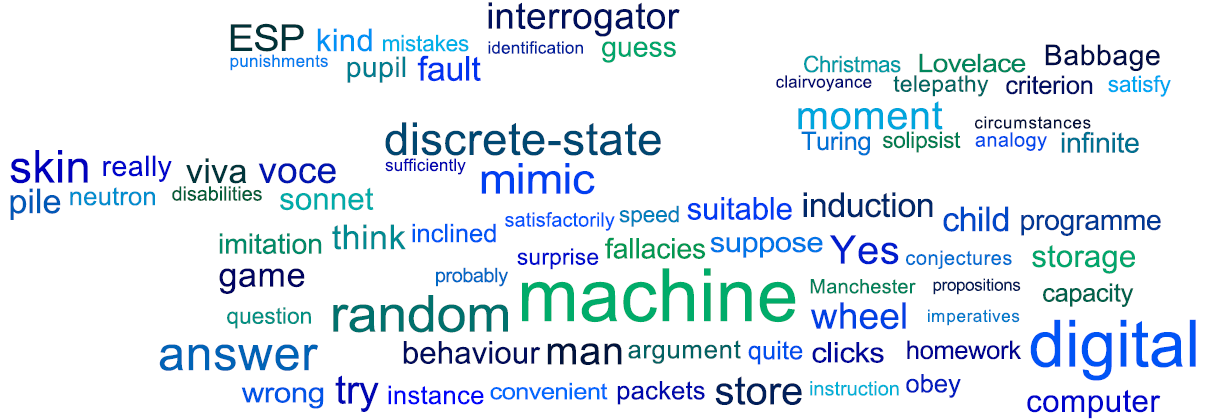
\includegraphics[scale=0.43]{img/wc_statiche/wc_semantic.png}
}

\frame{
\frametitle{\textbf{Word cloud dinamiche}\hspace{1mm}{\small(Cui et al., 2010)}}
\begin{center}
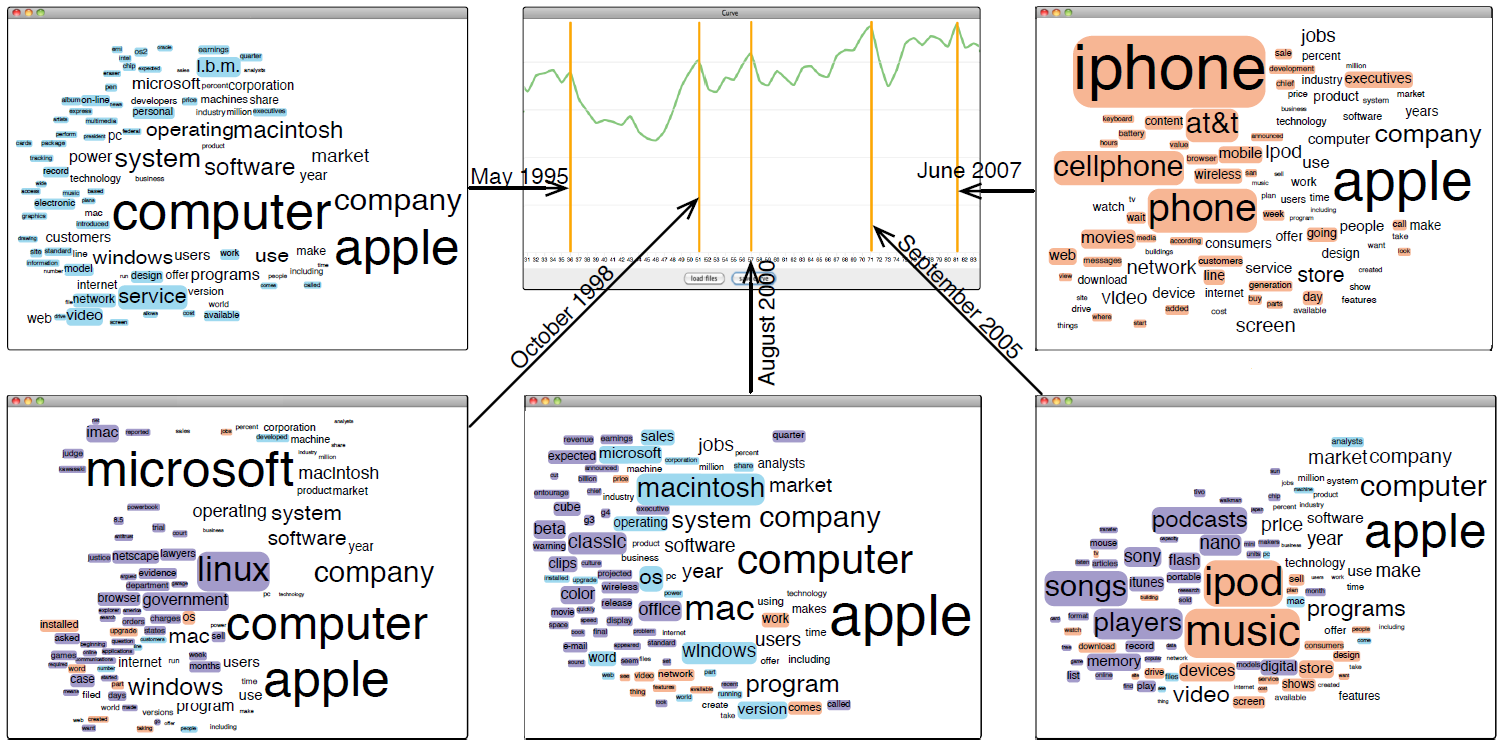
\includegraphics[scale=0.35]{img/wc_dinamiche/cui.png}
\end{center}
}
\frame{
\frametitle{\textbf{Morphing}\hspace{1mm}{\small(Chi et al., 2015)}}
\begin{center}
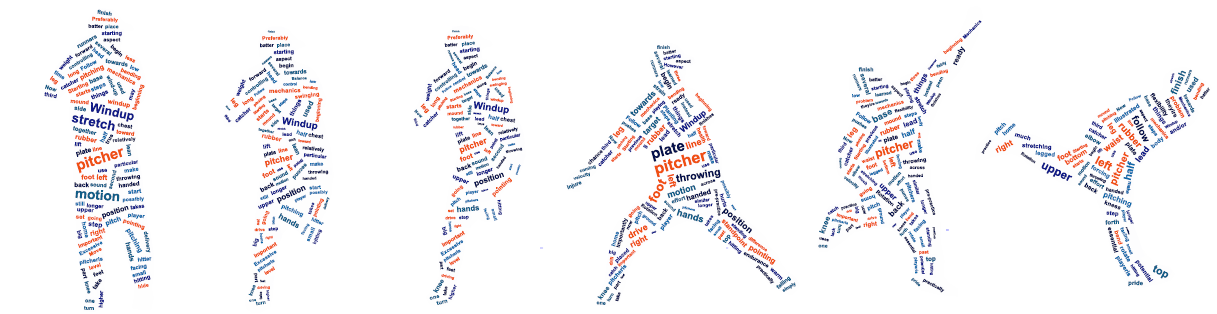
\includegraphics[scale=0.43]{img/wc_dinamiche/pitcher.png}
\end{center}
}

\section{Creazione word cloud}
\subsection{Word cloud statica}
\frame{
\frametitle{\textbf{Generazione word cloud semantica}}
\begin{beamerboxesrounded}[shadow=true]{}
	\begin{enumerate}
\item Estrazione parole chiave
\item Calcolo similarit�
\item Clustering
\item Disegno word cloud
	\end{enumerate}
\end{beamerboxesrounded}
}

\frame{
\frametitle{\textbf{Generazione word cloud semantica}}
\begin{beamerboxesrounded}[shadow=true]{}
	\begin{enumerate}[<+-| alert@+>]
\item <1| alert@+> Estrazione parole chiave
\item <2| alert@+> Calcolo similarit�
\item <3| alert@+> Clustering
\item <4| alert@+> Disegno word cloud
	\end{enumerate}
\end{beamerboxesrounded}
\begin{center}
\includegraphics<1>[scale=0.45]{img/wc_dinamiche/term_ext.png}
\includegraphics<2>[scale=0.45]{img/wc_dinamiche/matrix2.png}
\includegraphics<4>[scale=0.45]{img/wc_dinamiche/layout.png}
\includegraphics<3>[scale=0.5]{img/wc_dinamiche/clustering.png}
\end{center}
}

\subsection{Word cloud dinamica}
\frame {
\frametitle{\textbf{Generazione word cloud dinamica}}
Obiettivo: create $K$ word cloud dal testo, si vuole passare da una word cloud alla successiva in modo graduale tramite tecniche di morphing.
}

\frame {
\frametitle{\textbf{Morphing}}
\begin{beamerboxesrounded}[shadow=true]{Caratteristiche}
	\begin{itemize}
\item Numero di frame
\item Gestione stato delle parole
\end{itemize}
\end{beamerboxesrounded}
}

\frame{
\frametitle{\textbf{Stato delle parole}}
Le parole, tra una word cloud e la successiva, possono:
\begin{itemize}
\item<2> scomparire
\item<3> apparire
\item<4> rimanere nel layout (variando posizione)
\end{itemize}
\begin{center}
\includegraphics<3>[scale=0.75]{img/wc_dinamiche/new_word.png}
\includegraphics<2>[scale=0.75]{img/wc_dinamiche/disapp_word.png}
\includegraphics<4>[scale=0.6]{img/wc_dinamiche/morphcommon.png}
\end{center}
}

\frame {
\frametitle{\textbf{Generazione word cloud dinamica}}
\begin{beamerboxesrounded}[shadow=true]{Possibili problematiche}
	\begin{enumerate}
\item Variazione posizione delle parole
\item Variazione dei cluster
	\end{enumerate}
\end{beamerboxesrounded}
}

\frame {
\frametitle{\textbf{Generazione word cloud dinamica}}
\begin{beamerboxesrounded}[shadow=true]{Possibili problematiche}
	\begin{enumerate}[<+-| alert@+>]
\item <1| alert@+> Variazione delle parole
\item <2| alert@+> Variazione cluster
	\end{enumerate}
\end{beamerboxesrounded}
\includegraphics<1>[scale=0.42]{img/wc_dinamiche/layout_mod.png}
\includegraphics<2>[scale=0.45]{img/wc_dinamiche/clustersimil.png}
}

\frame{
\frametitle{\textbf{Architettura}}
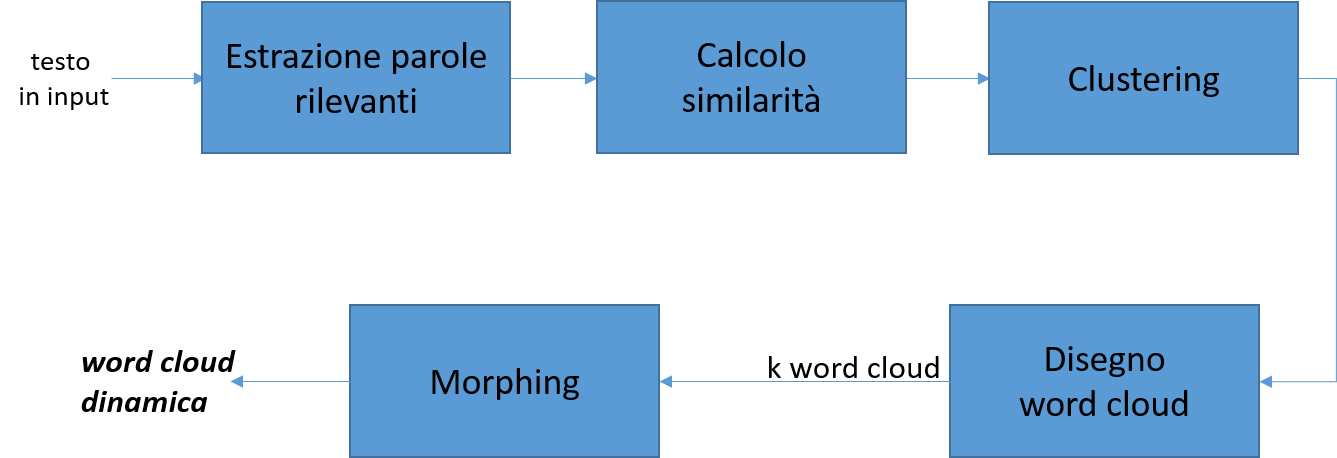
\includegraphics[scale=0.47]{img/wc_dinamiche/dynwc.png}
}

\frame{
\movie[width=11cm, height=6cm,start=1s, duration=24s, autostart, poster]{}{img/dynwc-1.avi}
}

\section{Risultati sperimentali}
\frame{
\frametitle{\textbf{Risultati sperimentali}}
Test suite: 
\begin{itemize}
\item $200$ discorsi estratti (file \textit{.txt}) dal set di conferenze annuali TED (Technology Entertainment Design).
\item Lunghezza media $17/18$ minuti.
\item 4 campionamenti per ogni testo.
\item Parole estratte: $20$,$40$,$60$
\end{itemize}
}

\frame{
\frametitle{\textbf{Risultati sperimentali}}
Metriche adottate:
\begin{itemize}
\item \textsf{Combination metric} $\, \Rightarrow  \nu = \dfrac{1}{K}\sum\limits_{k=1}^K (\alpha S^{k} + \beta\vartheta^{k,k-1}) $
	\begin{itemize}
	\item \textsf{Distortion metric} 
$\, \Rightarrow S^{k} = \dfrac{\sum \nolimits_{ij} c_{ij}s_{ij}}{\sum \nolimits_{ij} s_{ij}}$
	\item \textsf{Coherence metric }
$\,\Rightarrow  \vartheta^{k,k-1} = 1 - \dfrac{\sum \limits_{i=1}^p \sigma(w_{i}^{k},w_{i}^{k-1})}{pD} $
	\end{itemize}
\item \textsf{Space metric} $\Rightarrow  \gamma = 1 - \dfrac{\mu}{\varphi}$
\item \textsf{Tempo d'esecuzione}
\end{itemize}
}

\frame{
\frametitle{\textbf{Risultati sperimentali}}
Algoritmi utilizzati:
\begin{center}
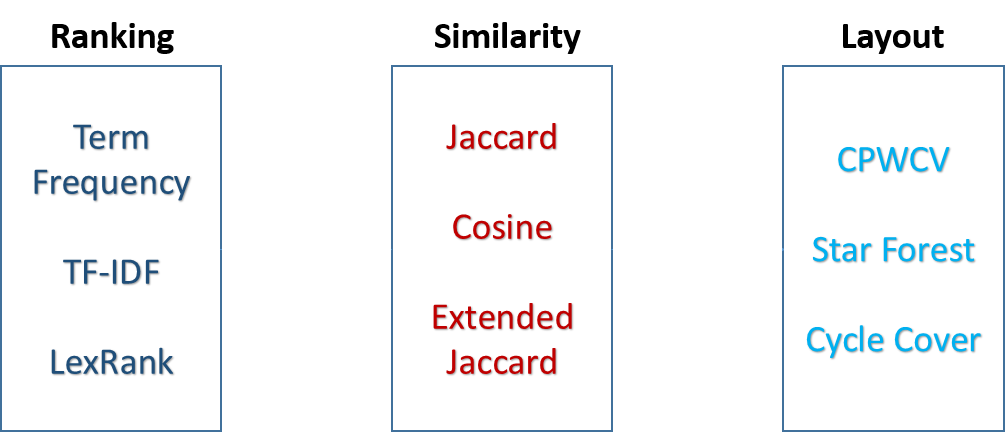
\includegraphics[scale=0.5]{img/wc_dinamiche/algorithms.png}
\end{center}
}

\frame{
\frametitle{\textbf{Combination metric}}
\includegraphics<1>[scale=0.25]{img/impl_test/test_tfidf_jaccard/figures/combo_20.png}
\includegraphics<2>[scale=0.25]{img/impl_test/test_tfidf_jaccard/figures/combo_40.png}
\includegraphics<3>[scale=0.25]{img/impl_test/test_tfidf_jaccard/figures/combo_60.png}

\only<1>{Parole estratte: 20}
\only<2>{Parole estratte: 40}
\only<3>{Parole estratte: 60}

Algoritmi utilizzati: TF-IDF Ranking, Jaccard Similarity
}

\frame{
\frametitle{\textbf{Space metric}}
\includegraphics<1>[scale=0.25]{img/impl_test/test_tfidf_jaccard/figures/spacemetric_40.png}

{Parole estratte: 40}

Algoritmi utilizzati: TF-IDF Ranking, Jaccard Similarity
}

\frame{
\frametitle{\textbf{Tempo d'esecuzione}}
\begin{itemize}
\item Configurazione caso peggiore: TFIDF, Jaccard Similarity e Star Forest
\item Configurazione caso migliore: Term Frequency, Cosine Similarity e CPWCV
\end{itemize} 
\tabcolsep=6mm
\resizebox{1\columnwidth}{!}   {
\begin{tabular}{ccc}
\hline
Parole estratte & Caso peggiore & Caso migliore  \\
\hline
$20$ & $2.65s$ & $0.77s$\\
$40$ & $3.01s$ & $0.94s$\\
$60$ & $3.66s$ & $1.25s$\\
\hline
\end{tabular}} 
}

\section{Conclusioni}
\frame{
\frametitle{\textbf{Conclusioni}}
\begin{itemize}
\item Nuovo approccio per la generazione di word cloud dinamiche.
\item Buoni risultati dagli algoritmi di layout utilizzati.
\item Tempo d'esecuzione soddisfacente. 
\end{itemize}
\vspace{0.1cm}
\setbeamercolor{postit}{fg=black,bg=green} %Baloon di colore diverso, senza sfondo
\begin{beamerboxesrounded}[upper=postit ,lower=postut ,shadow=true]{Sviluppi futuri:}
\begin{itemize}
\item Utilizzo di tecniche pi� sofisticate di Text Mining (e.g. \textit{POS Tagging}).
\item Definizione di metriche che tengano conto dell'interfaccia grafica + user study.
\end{itemize}
\end{beamerboxesrounded}
}

\frame{
\begin{center}
{\Large \textbf{Grazie per l'attenzione}}
\end{center}
}

\end{document}
